\documentclass[tikz,border=2pt]{standalone}
\usepackage{amsmath,amssymb}
\usepackage{pgfplots}
\pgfplotsset{compat=1.18}
\usetikzlibrary{calc}

\begin{document}
% Left: two independent fair dice; in every column the values of Y are 1..6 equally likely,
% so E[Y | X = x] = 3.5. Right: Y ~ Unif(-1,1), X = Y^2; the conditional mean is 0 for every x
% although X is a function of Y: a constant conditional mean does not give independence.
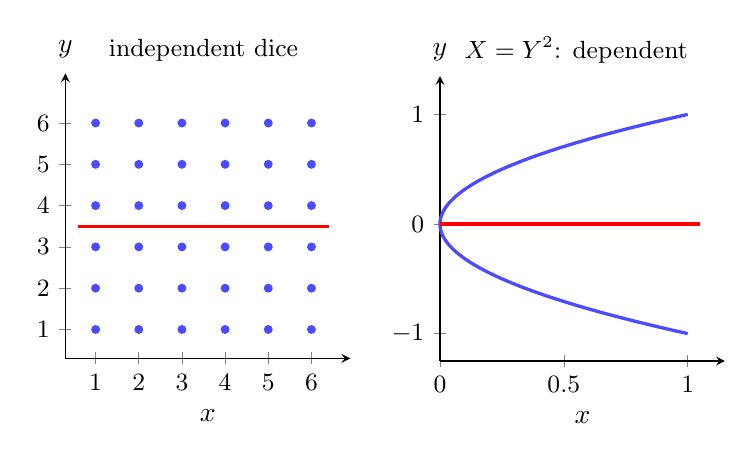
\begin{tikzpicture}
	\begin{axis}[
		name=dice, axis lines=left, xmin=0.3, xmax=6.9, ymin=0.3, ymax=7.2,
		xtick={1,...,6}, ytick={1,...,6}, tick label style={font=\small},
		xlabel={$x$}, ylabel={$y$}, ylabel style={rotate=-90, anchor=south, at={(axis description cs:0,1.02)}},
		width=5.2cm, height=5.2cm, clip=false
		]
		\addplot[only marks, mark=*, mark size=1.4pt, blue!70] coordinates {
			(1,1) (1,2) (1,3) (1,4) (1,5) (1,6) (2,1) (2,2) (2,3) (2,4) (2,5) (2,6) (3,1) (3,2) (3,3) (3,4) (3,5) (3,6)
			(4,1) (4,2) (4,3) (4,4) (4,5) (4,6) (5,1) (5,2) (5,3) (5,4) (5,5) (5,6) (6,1) (6,2) (6,3) (6,4) (6,5) (6,6)};
		\draw[red, very thick] (axis cs:0.6,3.5) -- (axis cs:6.4,3.5);
		\node[font=\small, anchor=south] at (axis cs:3.5,7.25) {independent dice};
	\end{axis}
	\begin{axis}[
		name=par, at={(dice.outer east)}, anchor=outer west, xshift=4mm,
		axis lines=left, xmin=0, xmax=1.15, ymin=-1.25, ymax=1.35,
		xtick={0,0.5,1}, ytick={-1,0,1}, tick label style={font=\small},
		xlabel={$x$}, ylabel={$y$}, ylabel style={rotate=-90, anchor=south, at={(axis description cs:0,1.02)}},
		width=5.2cm, height=5.2cm, clip=false
		]
		\addplot[blue!70, very thick, domain=-1:1, samples=80, variable=\t] ({\t*\t},{\t});
		\draw[red, very thick] (axis cs:0,0) -- (axis cs:1.05,0);
		\node[font=\small, anchor=south] at (axis cs:0.55,1.38) {$X=Y^2$: dependent};
	\end{axis}
	
\end{tikzpicture}
\end{document}
